\subsection{Inequalities, Intervals and Solving Basic Inequalities}\label{subsec:IneqInterval}

\subsection*{Inequality Notation}
Recall that we use the symbols $<,>,\leq,\geq$ when writing an inequality.
In particular,
\begin{itemize}
	\item $a<b$ means $a$ is to the \ifont{left} of $b$ (that is, 
				$a$ is \ifont{strictly less} than $b$),
	\item $a\leq b$ means $a$ is to the \ifont{left of or the same} 
				as $b$ (that is, $a$ is \ifont{less than or equal} to $b$),
	\item $a>b$ means $a$ is to the \ifont{right} of $b$ (that is, $a$ 
				is \ifont{strictly greater} than $b$),
	\item $a\geq b$ means $a$ is to the \ifont{right of or the same} 
				as $b$ (that is, $a$ is \ifont{greater than or equal} to $b$).
\end{itemize}

\noindent To keep track of the difference between the symbols, some students use the following mnemonic.\\

\begin{formulabox}[Mnemonic]
The $<$ symbol looks like a slanted \ifont{L} which stands for ``\ifont{L}ess than''.
\end{formulabox}

\bigskip

\begin{example}{Inequalities}{Inequalities}
The following expressions are true: 
\[ 1<2,\quad 
   -5<-2,\quad 
   1\leq 2,\quad
   1\leq 1,\quad
   4\geq\pi>3,\quad
   7.23\geq -7.23.
\]
\vspace{-0.5cm}
\end{example}

The real numbers are ordered and are often illustrated using the \dfont{real number line}:
\[

\includegraphics[width=5in]{images/real-number-line} 
\]

 
\subsection*{Intervals}
Assume $a,b$ are real numbers with $a<b$ (i.e., $a$ is strictly 
less than $b$). An \dfont{interval} is a set of every real number 
between two indicated numbers and may or may not contain the two numbers themselves.
When describing intervals we use both round brackets and square brackets.

(1) Use of round brackets in intervals: $(~,~)$.
The notation \dfont{(a,b)} is what we call the \dfont{open interval from a to b} 
and consists of all the numbers between $a$ and $b$, but does \ifont{not} include $a$ or $b$.
Using set-builder notation we write this as:
\[ (a,b)=\{x\in\mathbb{R}\,:\,a<x<b\}. \]
We read $\{x\in\mathbb{R}\,:\,a<x<b\}$ as ``the set of real numbers $x$ such that $x$ is greater than $a$ and less than $b$''
On the real number line we represent this with the following diagram:
\[

\includegraphics[width=2in]{images/interval-open} 
\]
Note that the circles on $a$ and $b$ are not shaded in, we call these \dfont{open circles} and use them to denote that $a$,$b$ are \ifont{omitted} from the set.

(2) Use of square brackets in intervals: $[~,~]$.
The notation \dfont{[a,b]} is what we call the \dfont{closed interval from a to b} 
and consists of all the numbers between $a$ and $b$ and \ifont{including} $a$ and $b$.
Using set-builder notation we write this as
\[ [a,b]=\{x\in\mathbb{R}\,|\,a\leq x\leq b\}. \]
On the real number line we represent this with the following diagram:
\[
\includegraphics[width=2in]{images/interval-closed} 
\]
Note that the circles on $a$ and $b$ are shaded in, we call these \dfont{closed circles} and use them to denote that $a$ and $b$ are \ifont{included} in the set.

To keep track of when to shade a circle in, you may find the following mnemonic useful:\\

\begin{formulabox}[Mnemonic]
The round brackets $(,)$ and non-shaded circle both form an ``O'' shape which stands for ``Open and Omit''.
\end{formulabox}

Taking combinations of round and square brackets, we can write different 
possible types of intervals (we assume $a<b$):
\[
\begin{array}{|c|c|c|}
\hline
(a,b)=\{x\in\mathbb{R}\,:\,a<x<b\} 
	& [a,b]=\{x\in\mathbb{R}\,:\,a\leq x\leq b\} 
	& [a,b)=\{x\in\mathbb{R}\,:\,a\,\leq x<b\}\\
	~&~&~\\

\includegraphics[width=1.8in]{images/interval-open} 
	& \includegraphics[width=1.8in]{images/interval-closed}
	& \includegraphics[width=1.8in]{images/interval-1}\\

\hline
(a,b]=\{x\in\mathbb{R}\,:\,a<x\leq b\}
	& (a,\infty)=\{x\in\mathbb{R}\,:\,x>a\} 
	& [a,\infty)=\{x\in\mathbb{R}\,:\,x\geq a\}\\
	~&~&~\\
\includegraphics[width=1.8in]{images/interval-2} 
	& \includegraphics[width=1.8in]{images/interval-3}
	& \includegraphics[width=1.8in]{images/interval-4}\\

\hline
(-\infty,b)=\{x\in\mathbb{R}\,:\,x<b\} 
	& (-\infty,b]=\{x\in\mathbb{R}\,:\,x\leq b\}
	& (-\infty,\infty)=\mathbb{R}=\mbox{all real numbers}\\
	~&~&~\\

\includegraphics[width=1.8in]{images/interval-5} 
	& 
\includegraphics[width=1.8in]{images/interval-6}
	& 
\includegraphics[width=1.8in]{images/interval-7}\\
\hline
\end{array}
\]

\textit{Note}: Any set which is bound at positive and/or negative infinity is an open interval.

\subsection*{Inequality Rules}
Before solving inequalities, we start with the properties and rules of inequalities.\\

%\begin{definition}{Inequality Rules}{Inequalityrules}
\begin{formulabox}[Inequality Rules]
{\bf Add/subtract a number to both sides:}\vspace{-0.2cm}
\begin{itemize}
	\item If $a<b$, then $a+c<b+c$ and $a-c<b-c$.
\end{itemize}
{\bf Adding two inequalities of the \red{same} type:}\vspace{-0.2cm}
\begin{itemize}
	\item If $a<b$ and $c<d$, then $a+c<b+d$.\\
				\ifont{Add the left sides together, add the right sides together.}
\end{itemize}
{\bf Multiplying by a \red{positive} number:}\vspace{-0.2cm}
\begin{itemize}
	\item Let $c>0$. If $a<b$, then $c\cdot a<c\cdot b$.
\end{itemize}
{\bf Multiplying by a \red{negative}  number:}\vspace{-0.2cm}
\begin{itemize}
	\item Let $c<0$. If $a<b$, then $c\cdot a>c\cdot b$.\\
		\ifont{Note that we reversed the inequality symbol!}
\end{itemize}
\end{formulabox}
%\end{definition}

Similar rules hold for each of $\leq$, $>$ and $\geq$.


\subsection*{Solving Basic Inequalities}
We can use the inequality rules to solve some simple inequalities. \\

\begin{example}{Basic Inequality}{BasicInequality}
Find all values of $x$ satisfying
\[ 3x+1>2x-3. \]
Write your answer in both interval and set-builder notation.
Finally, draw a number line indicating your solution set.
\end{example}

\begin{solution}
Subtracting $2x$ from both sides gives $x+1>-3$.
Subtracting $1$ from both sides gives $x>-4$.
Therefore, the solution is the interval $(-4,\infty)$.
In set-builder notation the solution may be written as $\{x\in\mathbb{R}\,:\,x>-4\}$.
We illustrate the solution on the number line as follows:
\[

\includegraphics[width=2in]{images/ineq-ex-1}
\]
\end{solution}

Sometimes we need to split our inequality into two cases as the next example demonstrates. \\

\begin{example}{Double Inequalities}{DoubleInequalities}
Solve the inequality 
\[ 4>3x-2\geq 2x-1. \]
\vspace{-0.5cm}
\end{example}

\begin{solution}
We need both $4>3x-2$ and $3x-2\geq 2x-1$ to be true:
\[\begin{array}{ccc}
	4>3x-2 & \mbox{\ifont{and}} & 3x-2\geq 2x-1,\\
	6>3x & \mbox{\ifont{and}} & x-2\geq -1,\\
	2>x & \mbox{\ifont{and}} & x\geq 1,\\
	x<2 & \mbox{\ifont{and}} & x\geq 1.\\
\end{array}\]
Thus, we require $x\geq 1$ but also $x<2$ to be true. 
This gives all the numbers between $1$ and $2$, including $1$ but not including $2$.
That is, the solution to the inequality $4>3x-2\geq 2x-1$ is the interval $[1,2)$.
In set-builder notation this is the set $\{x\in\mathbb{R}\,:\,1\leq x<2\}$.
\end{solution}

\bigskip

\begin{example}{Positive Inequality}{4x-inequality}
Solve $4x-x^2>0$.
\end{example}

\begin{solution}
We provide two methods to solve this inequality.

\bigskip
\noindent
\ifont{First method.} Factor $4x-x^2$ as $x(4-x)$.  The product of two numbers
is positive when either both are positive or both are negative, i.e., if
either $x>0$ and $4-x>0$, or else $x<0$ and $4-x<0$.  The latter alternative
is impossible, since if $x$ is negative, then $4-x$ is greater than 4, and
so cannot be negative.  As for the first alternative, the condition $4-x>0$
can be rewritten (adding $x$ to both sides) as $4>x$, so we need:
$x>0$ and $4>x$ (this is sometimes combined in the form $4>x>0$, or,
equivalently, $0<x<4$).  In interval notation, this says that the solution
is the interval $(0,4)$.

\bigskip
\noindent
\ifont{Second method.}  Write $4x-x^2$ as $-(x^2-4x)$, and then complete
the square, obtaining 
$$-\Bigl((x-2)^2-4\Bigr)=4-(x-2)^2.$$  
For this to be positive we need $(x-2)^2<4$, which means that $x-2$ must be less
than 2 and greater than $-2$:  $-2<x-2<2$.  Adding 2 to everything gives
$0<x<4$.  

\bigskip
\noindent
Both of these methods are equally correct; you may use either
in a problem of this type.
\end{solution}

We next present another method to solve more complicated looking inequalities.
In the next example we will solve a rational inequality by using 
a number line and test points. We follow the guidelines below.\\

\begin{formulabox}[Guidelines for Solving Rational Inequalities]
\begin{enumerate}\itemsep0em 
	\item Move everything to \ifont{one side} to get a $0$ on the other side.
	\item If needed, combine terms using a \ifont{common denominator}.
	\item \ifont{Factor} the numerator and denominator.
	\item Identify points where either the numerator or denominator is $0$. Such points
				are called \dfont{split points}.
	\item Draw a \ifont{number line} and indicate your split points on the number line. 
				Draw \ifont{closed/open circles} for each split point depending on 
				if that split point satisfies the inequality (division by zero is not allowed).
	\item The split points will split the number line into subintervals. For each 
				subinterval pick a \ifont{test point} and see if the expression in Step 3 
				is positive or negative. Indicate this with a $+$ or $-$ symbol on the 
				number line for that subinterval.
	\item Now write your answer in set-builder notation. Use the union symbol 
				$\cup$ if you have multiple intervals in your solution.
\end{enumerate}
\end{formulabox}

\begin{example}{Rational Inequality}{RationalInequality1}
Write the solution to the following inequality using interval notation:
\[\frac{2-x}{2+x}\geq 1.\]
\vspace{-0.5cm}
\end{example}

\begin{solution}
One method to solve this inequality is to multiply both sides by $2+x$, but because we do not know if $2+x$ is positive or negative we must split it into two cases (\ifont{Case 1:} $2+x>0$ and \ifont{Case 2:} $2+x<0$).

Instead we follow the guidelines for solving rational inequalities:
\[
\begin{array}{rcl}
\mbox{Start with original problem:}& ~ & \displaystyle{\frac{2-x}{2+x}\geq 1}\\
\\
\mbox{Move everything to one side:}& ~ & \displaystyle{\frac{2-x}{2+x}-1 \geq 0}\\
\\
\mbox{Find a common denominator:}& ~ & \displaystyle{\frac{2-x}{2+x}-\frac{2+x}{2+x} \geq 0}\\
\\
\mbox{Combine fractions:}& ~ & \displaystyle{\frac{(2-x)-(2+x)}{2+x} \geq 0}\\
\\
\mbox{Expand numerator:}& ~ & \displaystyle{\frac{2-x-2-x}{2+x} \geq 0}\\
\\
\mbox{Simplify numerator:}& ~ & \displaystyle{\frac{-2x}{2+x} \geq 0\quad(*)}\\
\end{array}
\]
Now we have the numerator and denominator in fully factored form.
The split points are $x=0$ (makes the numerator $0$) and $x=-2$ (makes the denominator $0$).
Let us draw a number line with the split points indicated on it:
\[
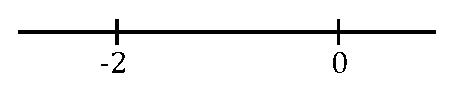
\includegraphics[width=2in]{images/ineq-rational-1}
\]
The point $x=0$ is included since if we sub $x=0$ into (*) we get $0\geq 0$ which is true.
The point $x=-2$ is not included since we cannot divide by zero.
We indicate this with open/closed circles on the number line (remember that open means omit):
\[

\includegraphics[width=2in]{images/ineq-rational-2}
\]
Now choosing a test point from each of the three subintervals we can determine if the expression $\frac{-2x}{2+x}$ is positive or negative.
When $x=-3$, it is negative.
When $x=-1$, it is positive.
When $x=1$, it is negative.
Indicating this on the number line gives:
\[

\includegraphics[width=2in]{images/ineq-rational-3}
\]
Since we wish to solve $\frac{-2x}{2+x}\geq 0$, we look at where the $+$ signs are and shade that area on the number line:
\[
\includegraphics[width=2in]{images/ineq-rational-4}
\]
Since there is a closed circle at $0$, we include it.
Therefore, the solution is $(-2,0]$.
\end{solution}

\begin{example}{Rational Inequality}{RationalInequality2}
Write the solution to the following inequality using interval notation:
\[ \frac{2}{x+2}>{3}{x+3}. \]
\vspace{-0.5cm}
\end{example}

\begin{solution}
We provide a brief outline of the solution.
By subtracting $(3x+3)$ from both sides and using a common denominator of $x+2$,
we can collect like terms and simplify to get:
\[ \frac{-(3x^2+9x+4)}{x+2}>0. \]
The denominator is zero when $x=-2$.
Using the quadratic formula, the numerator is zero when 
$x=\frac{-9\pm\sqrt{33}}{6}$ (these two numbers are approximately $-2.46$ and $-0.54$).
Since the inequality uses ``$>$'' and $0>0$ is false, 
we do not include any of the split points in our solution.
After choosing suitable test points and determining the sign of 
$\frac{-(3x^2+9x+4)}{x+2}$ we have
\[

\includegraphics[width=2.5in]{images/ineq-ex-2}
\]
Looking where the $+$ symbols are located gives the solution:
$$\left(-\infty,\frac{-9-\sqrt{33}}{6}\right)\bigcup\left(-2,\frac{-9+\sqrt{33}}{6}\right).$$
When writing the final answer we use \ifont{exact} expressions for numbers in mathematics, not 
approximations (unless stated otherwise).
\end{solution}
